% This is samplepaper.tex, a sample chapter demonstrating the
% LLNCS macro package for Springer Computer Science proceedings;
% Version 2.20 of 2017/10/04
%
\documentclass[runningheads]{llncs}
%
\usepackage{graphicx}
% Used for displaying a sample figure. If possible, figure files should
% be included in EPS format.
%
% If you use the hyperref package, please uncomment the following line
% to display URLs in blue roman font according to Springer's eBook style:
% \renewcommand\UrlFont{\color{blue}\rmfamily}

\begin{document}
%
\title{Contribution Title\thanks{Supported by organization x.}}
%
%\titlerunning{Abbreviated paper title}
% If the paper title is too long for the running head, you can set
% an abbreviated paper title here
%
\author{Guillermo Amorín\inst{1}\and
Second Author\inst{2,3}\orcidID{1111-2222-3333-4444} }
%
\authorrunning{G.Amorín et al.}
% First names are abbreviated in the running head.
% If there are more than two authors, 'et al.' is used.
%
\institute{Facutltad de Ingeniería, Universidad de la República, Montevideo Uruguay 
\email{gamorin@fing.edu.uy}}
%
\maketitle              % typeset the header of the contribution
%
\begin{abstract}
En el marco de la asignatura Taller de Sistemas Ciber-físicos dictada por el Instituto de Computación de la Facultad de Ingeniería - Universidad de la República, y en base al trabajo realizado por Reid Simmons, et.al. denominado Coordination for Multi-Robot Exploration and Mapping donde se presenta una utilización del estimador de información ganada al realizar exploración robótica, se pretende realizar un análisis sobre dicho estimador. En este trabajo, se presenta el problema de la exploración robótica, el trabajo de referencia consultados, los detalles de la solución propuesta para realizar los experimentos y se presentan los mismos junto con el análisis de resultados. A su vez, en base a los resultados obtenidos se plantean 2 hipótesis para orientar futuros trabajos. La primera es que a medida que la razón entre la información que un agente estima ganar al alcanzar un objetivo y la información realmente ganada, se aproxima a 1 y el robot se encuentra realizando la exploración en un entorno , es posible tomarlo como un indicador de que se está próximo al total de cubrimiento. Por último, la combinación de la utilización del indicador de información ganada con otro estimador puede provocar que la distancia recorrida por los agentes sea menor en comparación con la utilización de ambos indicadores por separado.

\keywords{Exploración robótica  \and Estimador de información ganada \and Utilidad.}
\end{abstract}
%
%
%

\section{Introducción}

El presente trabajo tiene como objetivo realizar un análisis sobre el aporte que realiza el estimador de información ganada al momento de la asignación de tareas en el problema de la exploración robótica multirobot.

Dicho análisis se basa en el aporte realizado por Reid Simmons, et.al. en el trabajo Coordination for Multi-Robot Exploration and Mapping \cite{artRef}, y se busca compararlo con otro estimador que tiene en cuenta solamente el costo en términos de distancia recorrida para llegar a determinado punto del mapa. 

A continuación, el documento se organiza de la siguiente manera: se presenta el problema de la exploración robótica con algunas de las múltiples aristas desde donde se puede atacar y se informa acerca de los trabajos revisados para la realización del trabajo. Luego se detalla la solución propuesta y se exponen las pruebas realizadas junto con sus resultados incluidos. Al final del documento se presentan las conclusiones obtenidas seguidas por las referencias revisadas.

\section{Presentación del Problema}

La exploración robótica es la tarea de construir un mapa que represente el entorno en que se encuentra el robot \cite{onSwitch}. En este escenario, el proceso de descubrir características del ambiente que rodea al el robot puede modelarse con la iteración de las siguientes actividades:
\begin{enumerate}
	\item Obtener información del entorno que lo rodea.
	\item Integrar la información percibida en un mapa que represente lo conocido por el robot hasta el momento.
	\item Decidir la siguiente localización a donde debe dirigirse.
	\item Alcanzar esa localización.
\end{enumerate}

Dicho proceso puede ser mas efectivo al realizarse en paralelo por mas de un robot, dividiendo las tareas en subtareas y ejecutándolas en paralelo. Un equipo de robots puede hacer uso de especialistas (agentes que recolecten información sobre la frontera de la exploración, otro que muevan objetos, etc) y/o tener agentes que se utilicen para varias tareas y no sean expertos en ninguna\cite{war}.

Esta perspectiva de utilizar varios agentes no nos modifica el modelo planteado anteriormente para un único agente sino que lo paraleliza y aplica para cada agente.


Al trabajar en un ambiente desconocido con la ausencia de un mapa, la navegación y planificación de tareas debe realizarse en función de la información obtenida hasta el momento y el sensado local realizado, por lo que la exploración del ambiente se logra en base a soluciones no optimas o localmente optimas. La construcción del mapa de un ambiente desconocido debe realizarse de manera incremental, donde la estrategia de búsqueda (en referencia a la de nueva información para completar el mapa) o la planificación de tareas basadas en el sensado de características del ambiente son muy importantes. Por lo tanto mientras mas preciso y completo sea el sensado de los agentes mas beneficioso sera para la construcción del mapa\cite{cooperative2017}.

Para representar un mapa existen principalmente 2 posibles enfoques, geométrico o topológico. En el primero los objetos se representan mediante su relaciones geométricas absolutas, por ejemplo en la forma de una grilla de ocupación, mapa de polígonos o un mapa de lineas. La principal ventaja de estos mapas es que proveen información métrica muy precisa pero generan dificultades a la hora de mantenerlos a grandes escala, planificar o generar trayectorias. Los segundos son mapas que se basan en características del ambiente que se obtienen del sensado y carecen de cualquier relación métrica, sin embargo la relación entre puntos característicos es mantenida. Estos mapas son difíciles de mantener si la información obtenida del esquema de sensado de los agentes es vaga\cite{cooperative2017}. Existen a su vez otros tipos de mapas como se plantea en\cite{Luo}, el cual combina una representación de un mapa de grilla con varios niveles con las características obtenidas mediante sensado de imágenes por parte del agente. En la Figura \ref{Figura Entornos} se muestra una representación de un mismo ambiente desde los 3 enfoques presentados.

\begin{figure}
	\centering
	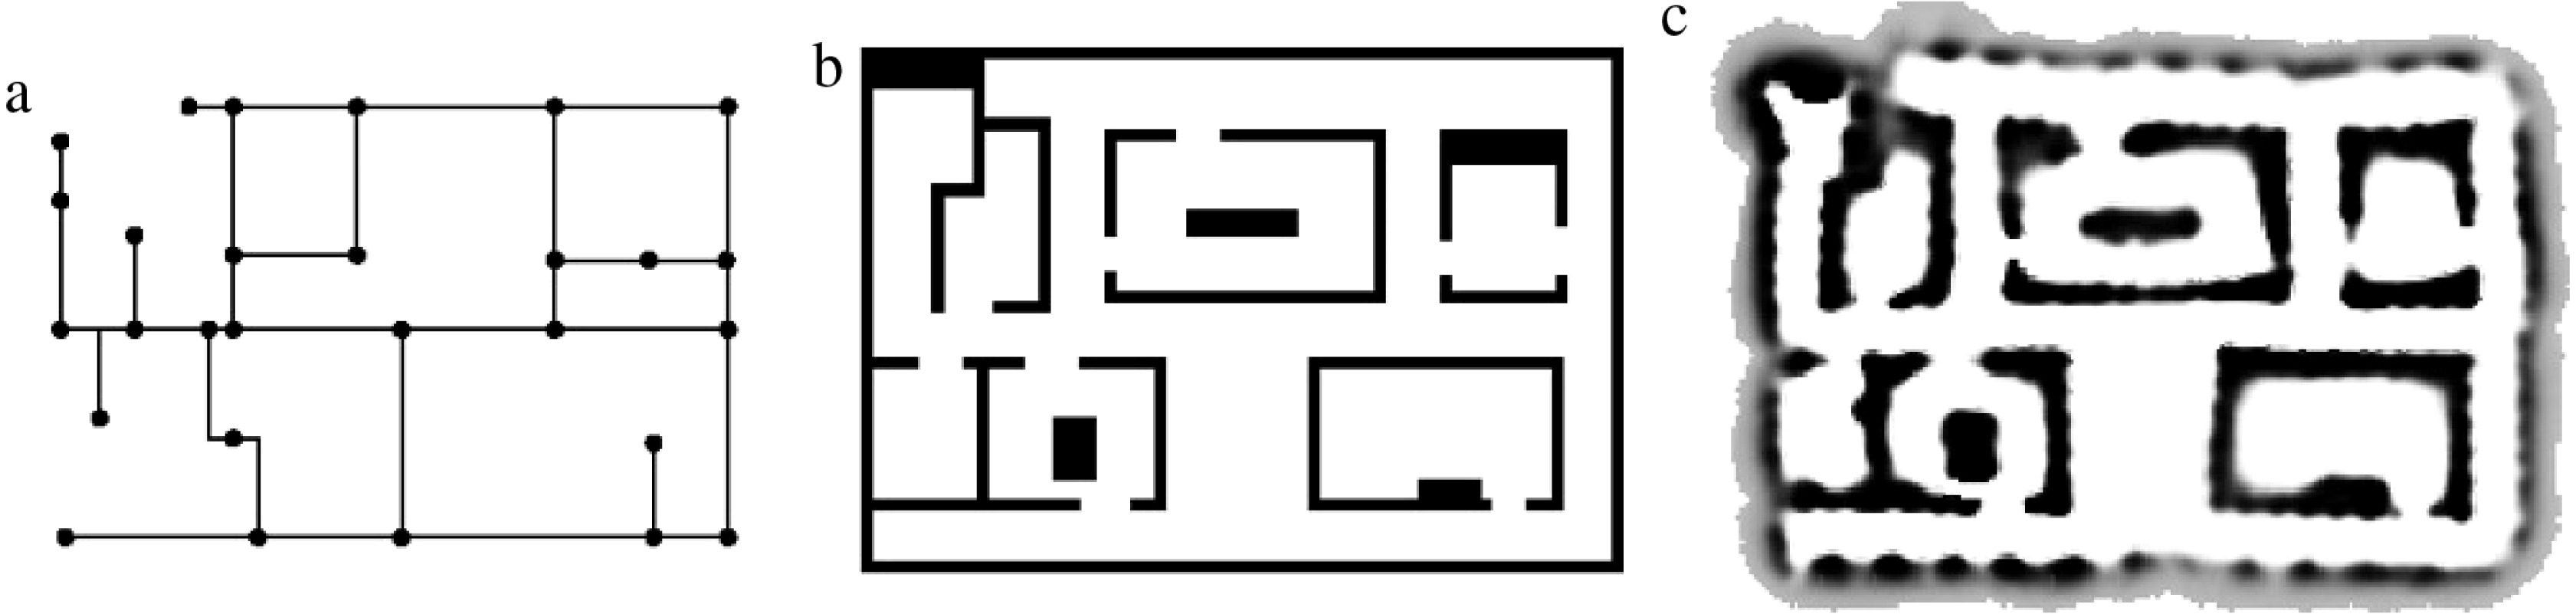
\includegraphics[height=0.75in]{./Imagenes/Imagen1.jpg}
	\caption{Imagen tomada de \cite{artRef}, Derecha: Mapa topológico, Centro: Mapa gemonétrico, Izquierda: combinación}
	\label{Figura Entornos}
\end{figure}

Para la combinación de información sensada así como de múltiples mapas existen 2 enfoques principales, el basado en puntos y el basado en características.\cite{lu} El basado en puntos analiza punto a punto la información existente y mediante un mecanismo de combinación (p.e.: preferencia o probabilista) agrega la información del punto al mapa que está construyendo. El basado en características en lugar de trabajar con las medidas en crudo, las transforma en características del ambiente y las unifica con las características existente y sus relaciones\cite{cooperative2017}.

La principal dificultad de la exploración multirobot es la coordinación de la ejecución de las distintas tareas de los robots\cite{war}, la importancia de aplicar una buena estrategia al asignar las distintas tareas puede verse en\cite{fontan} y \cite{tool} donde múltiples agentes obtienen peores resultados en términos de tiempo de exploración debido a la interferencia entre ellos que al realizar la exploración con un solo agente.

Como dice \cite{war} un enfoque para llevar adelante la estrategia de exploración consiste en considerar al equipo de agentes como una sola entidad con muchos grados de libertad, donde un centro de computo de manera centralizada computa la manera optima de ejecutar las distintas tareas. Los mejores algoritmos para realizar dicho computo son de complejidad exponencial y por lo tanto son intratables para equipos de muchos robots. Ademas por lo general se asume que la información puede llegar de cualquier lugar del mapa a este modulo central para que distribuya las tareas y que esta información no cambia en ese trayecto \cite{war}, lo cual es una asunción que escapa un poco a la realidad, principalmente por los problemas de conectividad. Otra desventaja de este enfoque es que la coordinación de los robots depende de un solo individuo, que si falla el sistema corre riesgo de colapsar a menos que exista una rutina de sustitución.

Otro enfoque es el presentado en \cite{otro} donde la distribución de tareas se realiza de forma descentralizada y cada robot toma la decisión de a donde dirigirse en función de la información que dispone y siguiendo un protocolo utilizando su propia capacidad de computo.

Una cuestión transversal ya sea en la coordinación centralizada o descentralizada es la forma en que se determina cuan conveniente es ir a determinado lugar de la zona explorada para continuar con la exploración. Esto puede realizarse teniendo en cuneta diversas cuestiones como por ejemplo la distancia que es necesario recorrer, la cantidad de agentes cercanos a dicha posición, la posibilidad de interferir en el trayecto de otro agente, la información que posiblemente pudiera llegar a ganar el robot de alcanzar dicha posición, o cualquier otro aspecto que quien desarrolle el sistema de coordinación considere pertinente. Sujeto a que aspectos son considerados, aumenta o disminuye la efectividad de la estrategia

En \cite{metricas} se mencionan varias de las métricas utilizadas al realizar exploración robótica. Alguna de ellas son:

\begin{itemize}
	\item tiempo de exploración
	\item costo en termino de distancia (sima de la distancia recorrida por cada robot)
	\item eficiencia, donde la define como el Area explorada en metros cuadrados dividida el costo de la exploración.
\end{itemize}


\section{Trabajos relacionados}

Esta sección se presenta principalmente un análisis del artículo en el cual se basó el trabajo realizado, “Coordination for Multi-Robot Exploration and Mapping”(en adelante el artículo de referencia). Dicho artículo desarrolla una técnica de exploración donde múltiples y heterogéneos agentes tiene el objetivo de explorar un ambiente grande en superficie e interior, considerando 2 problemas principales:
Crear un único mapa global a partir de la información sensada por cada agente.
Y decidir a que lugar se debe dirigir cada agente para realizar la exploración de la manera mas eficiente posible.

Para atacar el punto 2 los autores tiene en cuenta el indicador de información ganada, que se  estima como la información nueva que se obtendrá luego de que un robot alcance un objetivo determinado. Si bien para determinar cuanta información se obtiene al alcanzar un objetivo es necesario saber cuanta información se obtuvo a lo largo de todo el trayecto. Esto es muy costoso \cite{utility} y por eso varios trabajos \cite{Visser, Zlot, Gonzalez} lo estiman solamente como la información que se obtiene al llegar al objetivo final de la tarea.

A continuación se divide esta sección en 4 subsecciones para describir el trabajo de referencia: aspectos generales, enfoque utilizado para la creación del mapa global, enfoque utilizado para la distribución de tareas y las conclusiones a las que arribó el trabajo.

\subsection{Consideraciones generales}

La comunicación entre robots y en caso de que exista con una estación base o módulo central es muy importante al momento de realizar la exploración por las restricciones que esta introduce al trabajar fuera del simulador en un ambiente físico. Blach y Arkin \cite{Blach} estudian como afecta la comunicación en los sistemas multirobot, particularmente en la tarea de explorar el 100 \% del ambiente. Haciendo que los robots decidan los lugares a donde ir de manera aleatoria logran resultados menos efectivos(en términos de tiempo de exploración) en comparación con los realizados en trabajo de referencia, si bien no se realizan comparaciones explicitas. 

Como ya se mencionó antes, Singh y Fujimura \cite{otro} presentan un enfoque descentralizado para agentes heterogéneos. Aquí cada agente decide por si mismo donde debe dirigirse, pero cunado se encuentra con un pasaje donde por su tamaño le es imposible acceder, selecciona otro agente del sistema de menor tamaño para que explore dicha área. Esta selección es realizada en base a la distancia entre los agentes y el área objetivo, los tamaños de los agentes, y la cantidad de áreas exploradas por los agentes.

Un artículo que introduce el concepto de frontera, concepto importante sobre el cual se apoyan fuertemente el trabajo de referencia y el realizado, es \cite{Yama} donde Yamauchi desarrolla una técnica en la cual múltiples robots genera un único mapa en forma distribuida. El trabajo define una celda de frontera ( en un mapa de grilla ) como el una celda conocida que tienen al menos una celda vecina desconocida. Esta noción es utilizada para determinar las distintas fronteras en un mapa, de las cuales se determinan los puntos más representativos y es entre esos puntos, donde los robots deciden a donde dirigirse. Es importante destacar que los robots lo hacen de manera independiente pudiendo así dirigirse 2 o más robots a la misma localización, lo cual genera ineficiencia.

\subsection{Enfoque para la creación del mapa global}

Para realizar la creación del mapa global en el trabajo de referencia se realizan 2 suposiciones, una basada en en varios trabajos de la literatura relacionada como \cite{thrun, leo, choset} y consiste en asumir que el entorno es lo suficientemente estático. La otra es que los robots inicialmente saben sus posiciones relativas ya que inician de posiciones donde se detectan mutuamente. Esto se realiza con el fin de simplificar el problema de estimar las posiciones relativas.

Para la construcción de un mapa local, cada robot toma un conjunto de medidas a partir de sus sensores y estima su posible ubicación en su mapa local maximizando una función de probabilidad que tiene en cuenta un modelo del ruido de la odometría y de la percepción de los sensores. Ademas cada robot selecciona un subconjunto de las medidas tomadas y se las envía a un módulo central para que realice un mapa global. 

El módulo central para realizar el mapa, utiliza el mismo algoritmo que se aplica en cada agente independiente, y estima de la misma forma las distintas ubicaciones de los agentes para integrar la información e ir construyendo un mapa global. 

Según los autores la forma de construcción integra los distintos mapas de manera consistente y con relativamente poca exigencia de computo.

\subsection{Enfoque para la coordinación de agentes}

El objetivo de la coordinación de agentes es maximizar la información ganada, es decir el conocimiento del mapa. Para eso cada robot luego de actualizar su mapa, construye ofertas para enviar a un módulo central que conciten en la utilidad de trasladarse a varios puntos del mapa. Luego mediante una técnica de relativo bajo costo computacional y teniendo en cuenta el solapamiento de las áreas descubiertas, el módulo central asigna a donde debe dirigirse cada robot. 

Una oferta es una lista del costo y la información ganada de visitar una celda de frontera. Para mejorar el rendimiento, los autores estipularon que una celda de frontera que posiblemente sea visitada deba estar a una distancia mínima de cualquier otra celda que pueda llegar a ser visitada, o exista un obstáculo entre 2 celdas de frontera. Con esto se logra que 2 celdas de frontera que están muy cerca en distancia pero separadas por una pared sean consideradas ambas en la lista.

Para estimar el costo de visitar una celda, se calcula el camino mínimo a dicha celda y se computa como el costo. La información ganada se calcula mediante la cantidad de celdas desconocidas que se encuentran en el rango de sensado del agente si este estuviese localizado en la celda de frontera. Ademas al calcular la información ganada, los autores calculan un rectángulo que aproxima dicha magnitud con el fin de facilitar los cálculos de la superposición de las áreas obtenidas al visitar distintos puntos. En la figura \ref{Figura IGR} se representar la zona de sensado con una circunferencia, dentro de esta se indican con cruces lo que corresponde a información ganada y la línea punteada se refiere a los rectángulos de aproximación del área de información ganada (en adelante IGR). También es posible observar en dicha imagen la superposición de las áreas de información ganada.

\begin{figure}
	\centering
	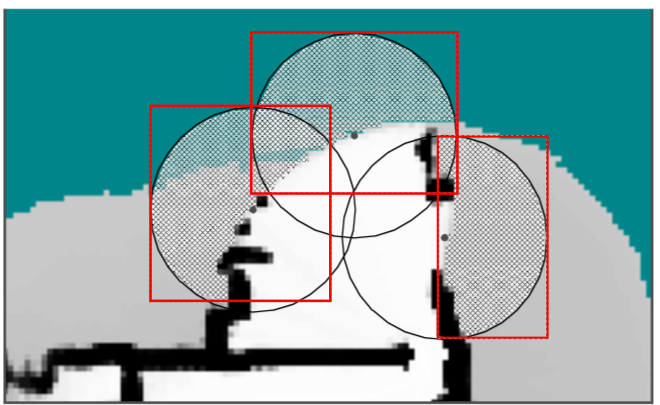
\includegraphics[height=1.5in]{./Imagenes/Imagen2.png}
	\caption{Imagen tomada de \cite{artRef}, En rojo los IGR, marcado con cruces se encunetra la información ganada.}
	\label{Figura IGR}
\end{figure}

\subsection{Enfoque para la asignación de tareas}

Para la asignación de tareas se utiliza un algoritmo sencillo con el fin de mantener el costo computacional bajo y lograr realizar la asignación en tiempo real. Los robots envían ofertas de forma asincrónica a el módulo central. Luego de un tiempo de recibir la primer oferta el módulo central toma todas las ofertas recibidas y asigna las tareas de acuerdo a la utilidad (información ganada menos el costo) de cada una. Esto lo hace de la siguiente manera, primero busca entre todas las ofertas aquella que obtiene mayor utilidad y le asigna ese objetivo al agente que origino la oferta. Luego actualiza las ofertas, multiplicando la utilidad por un valor correspondiente al porcentaje de superposición que tiene cada una con la información que ganaría el agente al cual se le asignó una tarea de cumplir con la misma y nuevamente comienza a buscar entre las ofertas actualizadas la que brinda mayor utilidad. Esto continua hasta que no haya mas ofertas que asignar o hasta que todos los agentes que enviaron ofertas se encuentren asignados.

Un aspecto clave en la asignación es el cálculo del porcentaje de solapamiento entre las áreas de información ganada ya que sin el los robots no tendrían coordinación alguna. Para calcular este solapamiento, los autores lo utilizan los IGR ya que esto les cuesta menos capacidad de cómputo y lo realizan de la siguiente manera:

\begin{center}
	$d_j = \frac{Area(IGR_j \cap ( \cup IGR_i , i \epsilon R))}{Area (IGRj)}$
\end{center}

\begin{center}
	$u_j = (1 - d_j) \times i_j - c_j $
\end{center}

Aquí, IGRj es la aproximación rectangular de la información ganada para la celda j. IGRi son los rectángulos de información ganada para los robots que ya fueron asignados, conjunto  R, e ij y cj son la información ganada que espera obtener el robot que origina la oferta y el costo del camino mínimo para llegar a ella respectivamente. 

Un factor importante en el calculo de la información ganada es la histéresis. Este valor es un factor que utiliza cada robot como divisor de la información ganada que este calcula para ir a un lugar en el mapa, cada vez que dicho lugar cae en el área de la información ganada de su objetivo actual. Este factor es un número entre 0 y 1, por lo general 0,85. Mientras mas bajo sea la histéresis, menor será la disposición del robot a cambiar de objetivo. El objetivo principal de incluir este factor es que como los agentes están continuamente sensando, la información ganada puede cambiar drásticamente luego de pequeños movimientos. Por ejemplo al encontrarse con una pared en lo desconocido. Esto se observa cunado un robot maniobra frente a una puerta, típicamente descubre una gran porción del cuarto, y sin la histéresis el robot no le encontraría mucha utilidad a la exploración completa de cuarto.

\subsection{Experimentos y Conclusiones}

Los experimentos se realizaron en distintos ambientes (2 ambientes de oficinas, un ambiente libre de obstáculos y 2 ambientes con obstáculos al azar, Ver Figura \ref{Figura Entornos 345}) con hasta 3 robots, 2 Pioneer AT de RWI y un Uribe de IS Robotics. El número de robots fue cambiando de 1 a 3 y en base a eso se compararon los resultados entre utilizar uno o varios robots. 

Si bien los resultados obtenidos muestran una mejora en el tiempo total de exploración y la precisión del mapa de múltiples robots en comparación con uno solo, los autores no pudieron cuantificar otros factores resultado de las decisiones de diseño como: el efecto de la histéresis, el error en el calculo del solapamiento de la información ganada, o la definición de la información ganada. 

\begin{figure}
	\centering
	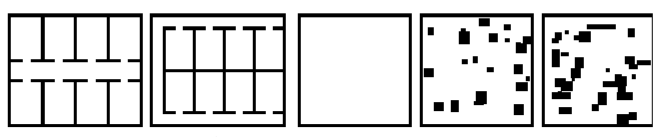
\includegraphics[height=0.70in]{./Imagenes/Imagen3.png}
	\caption{Imagen tomada de \cite{artRef}, Entornos utilizados en el artículo de referencia}
	\label{Figura Entornos 345}
\end{figure}


\section{Solución propuesta}

La solución aquí planteada busca en base al trabajo realizado en el artículo de referencia poder comparar la asignación de tareas utilizando el indicador de información ganada y una asignación de tareas utilizando un indicador de costo, tomando como costo la distancia que recorrería el agente en caso de tener que ir a un objetivo determinado. Ademas, al realizar simulaciones con el estimador de información ganada interesa saber cuantas veces la decisión tomada con este estimador hubiera sido distinta a tomar la decisión por costos, y en esas ocasiones cuanta fue la información ganada en relación a la estimación que se realizó para asignar la tarea.

Este análisis se realiza en un marco de trabajo similar al artículo de referencia pero con algunas simplificaciones a modo de facilitar la obtención de la información previamente mencionada. La principal diferencia es que los experimentos se realizaron utilizando un simulador, el resto serán mencionadas a medida que se va detallando la solución propuesta.

La representación del mapa que se utilizó para realizar el trabajo es un mapa de grilla, donde las celdas pueden tener valor 0,100,-1 y representan vacío, ocupado y desconocido respectivamente. Las celdas vacías u ocupadas en ocasiones se pueden calificar como conocidas.

\subsection{Arquitectura de la solución}

Para realizar los experimentos y las pruebas, se utilizó un marco de trabajo similar al planteado en el trabajo \cite{metricas} donde se utiliza el simulador MORSE \footnote{https://www.openrobots.org/wiki/morse} para simular un ambiente real, pero en nuestro caso es configurado para obtener en cada momento de tiempo la ubicación exacta de cada agente, y la información de sensado sin error. Dicho simulador se comunica con módulos externos desarrollados en C++ a través de 2 interfaces distintas, por sockets para controlar la navegación de cada robot, y poder utilizar las librerías del simulador que se encargan de la navegación mediante waypoints. La segunda interfaz utilizada es ROS \footnote{www.ros.org}, con la cual se provee un entorno donde el simulador publica información sobre el ambiente y esta es consumida por un módulo central, los agentes y el monitor que determina el fin de la exploración.  Gracias a la utilización de esta interfaz, se facilita también la comunicación entre módulos, y la misma se realiza mediante ROS. 

La solución se integra por 3 componentes principales ademas del simulador, uno donde se implementa el componente  central, el cual asigna tareas y realiza la construcción del mapa global, otro que se divide en varios módulos e implementa la lógica de funcionamiento de cada robot y por ultimo un componente que funciona a modo de control, el cual es quien determina el fin de la exploración. Ver Figura \ref{Arqui}. Cada agente luego se controla con una instancia del segundo componente.

\begin{figure}
	\centering
	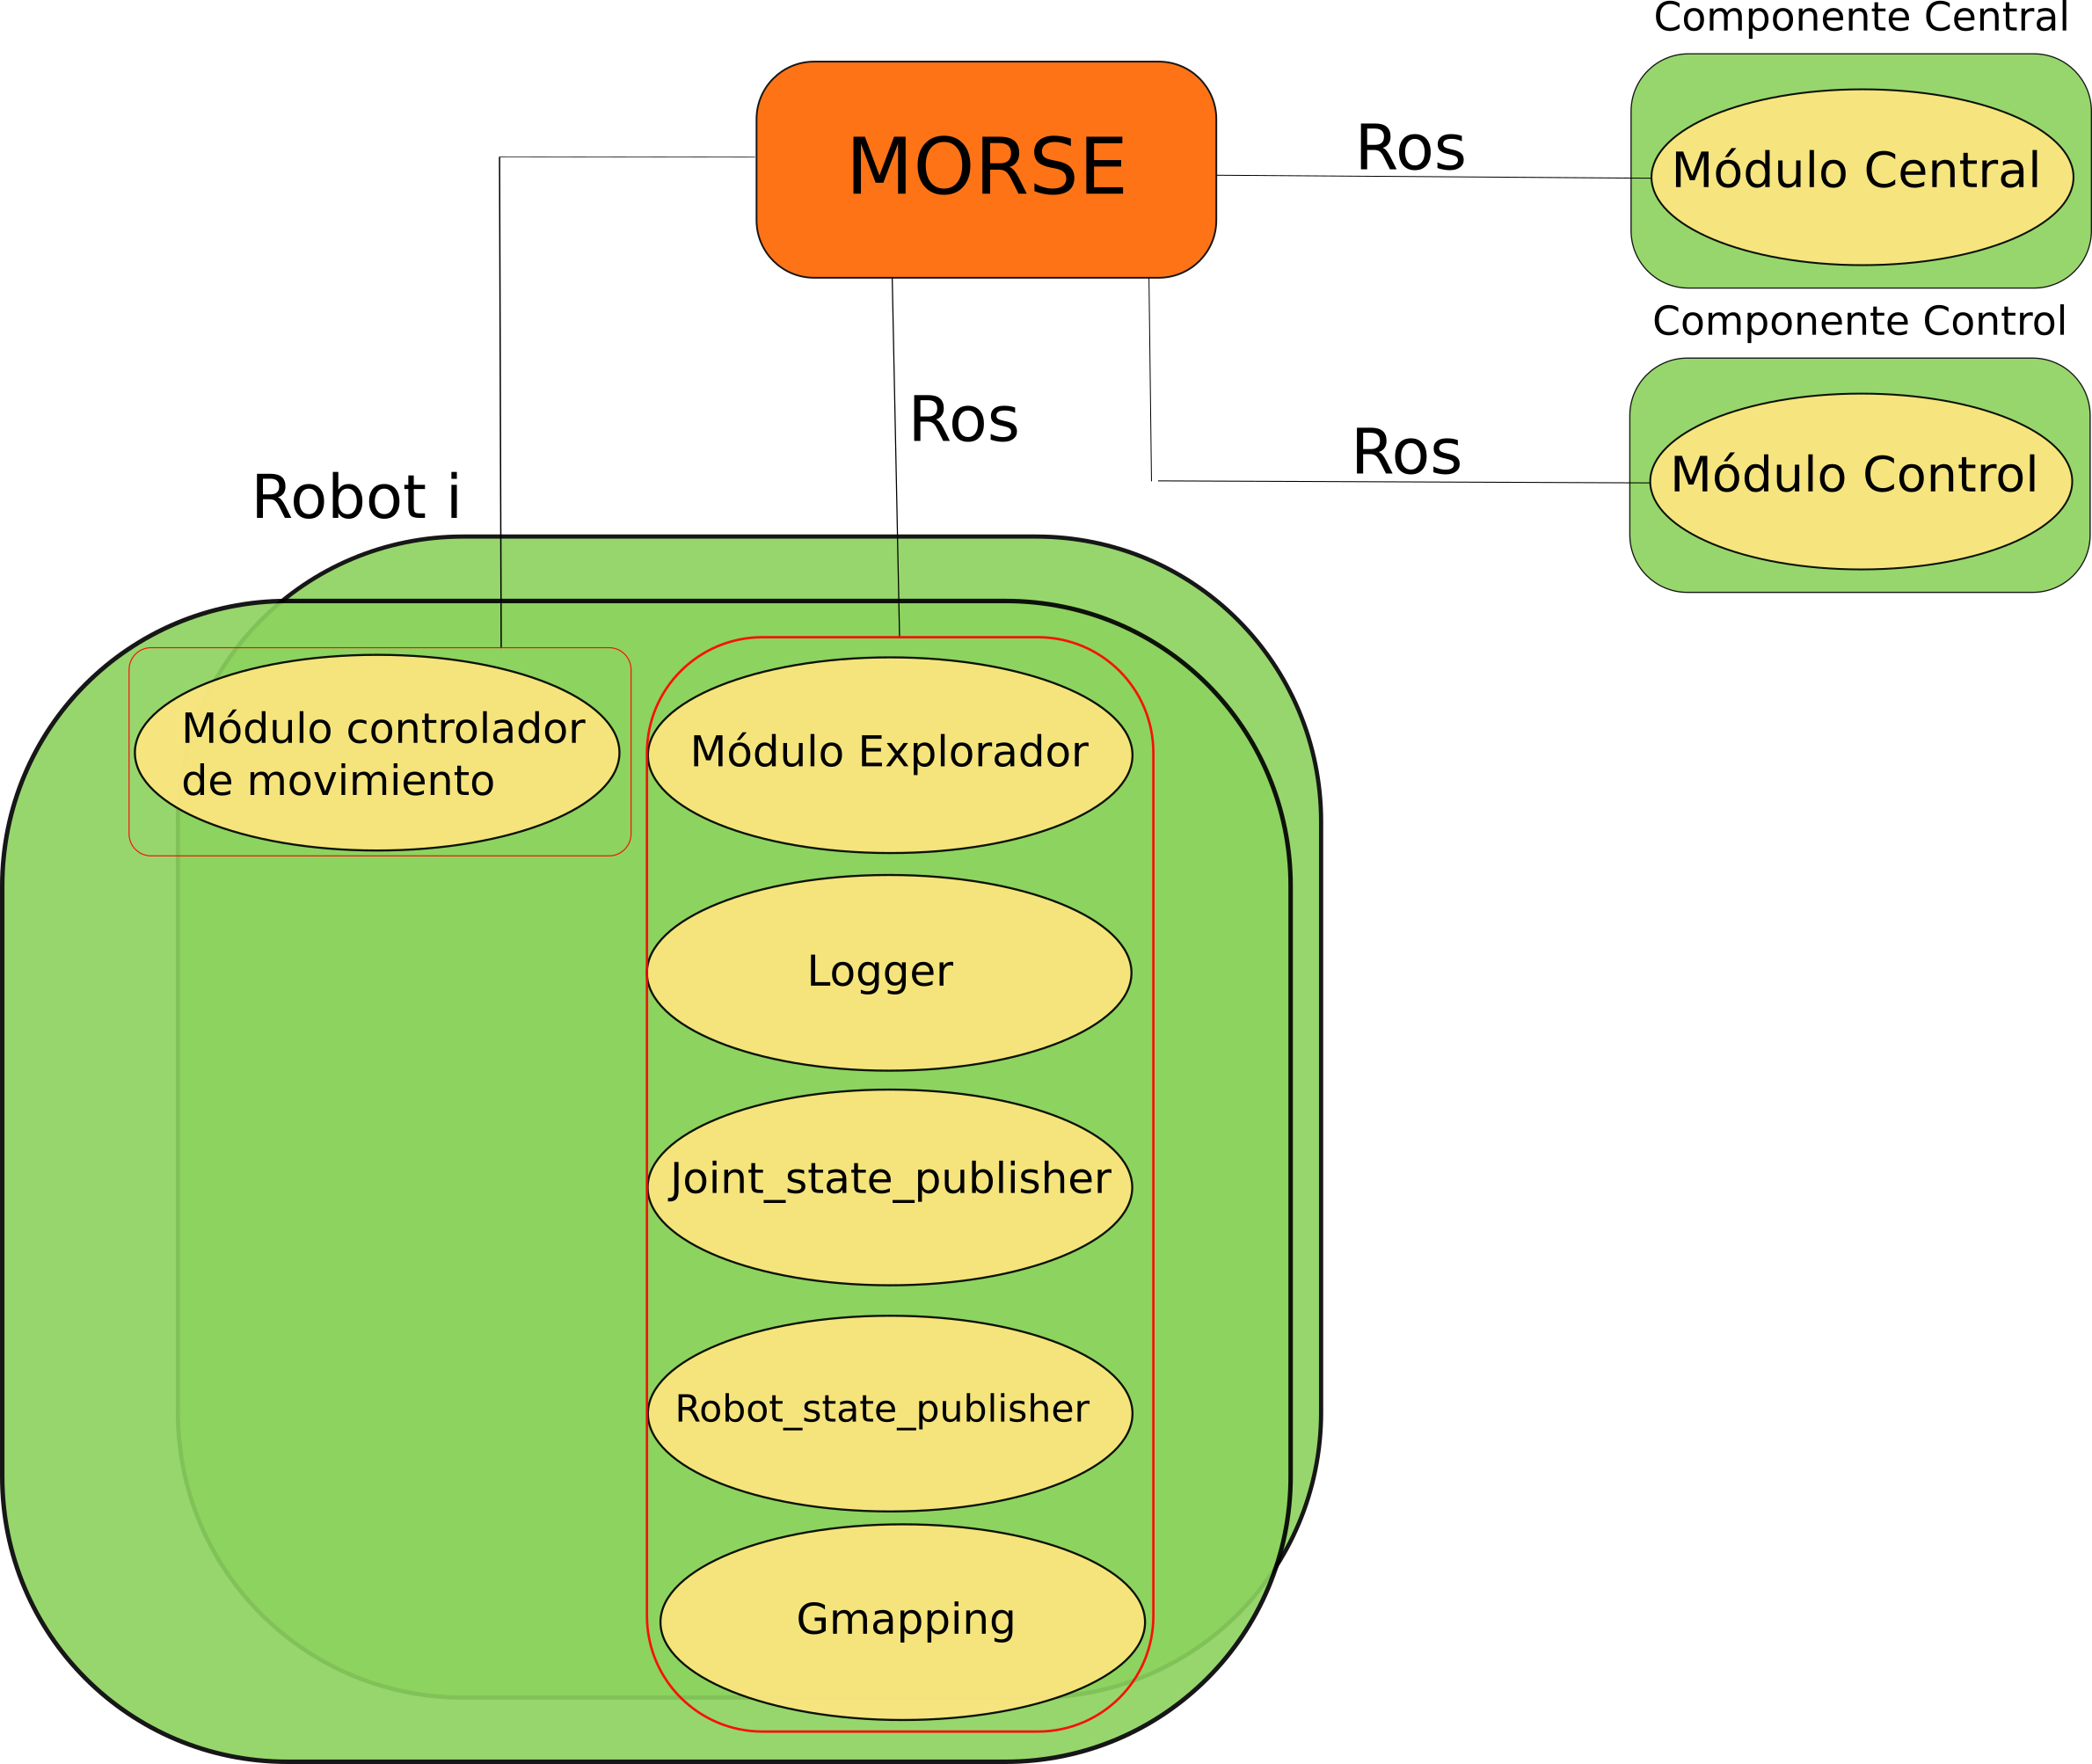
\includegraphics[height=2.5in]{./Imagenes/arqui.png}
	\caption{Imagen propia, Arquitectura de la solución}
	\label{Arqui}
\end{figure}

\subsection{Componente central}

Este módulo se encarga de varias cosas en paralelo, mantener la posición actual de cada robot, realizar la construcción del mapa global, y esperar reportes del alcance de los objetivos para realizar la asignación de tareas.

Para mantener la posición actual, el módulo central lee de los distintos topicos publicados por el simulador con la posición exacta de cada agente y la almacena en memoria. 

Esa posición se utiliza luego en la construcción del mapa global, ya que para cada mapa publicado por los distintos agentes, el módulo central con la posición del mismo analiza la porción del mapa que se encuentra en un radio de 8 metros con centro en la posición del agente al momento de publicar el mapa y con eso actualiza el mapa global. El algoritmo implementado para realizar esta construcción es el siguiente:

\begin{itemize}
	\item Para cada mapa publicado por el agente i:
	\begin{itemize}
		\item Para cada celda cuya distancia es menor a 8 metros de la posición del agente i:
		\begin{itemize}
			\item si la celda del mapa global es desconocida o sino existe un agente más cercano a dicha celda
			\begin{itemize}
				\item el valor de dicha celda pasa a ser el calor de la misma celda en el mapa publicado
			\end{itemize}
			\item sino
			\begin{itemize}
				\item el valor en el mapa global se mantiene
			\end{itemize}
		\end{itemize}
	\end{itemize}
\end{itemize}

Este algoritmo se construyó en base a el implementado por Z.Yan et.al. en el trabajo \cite{chino} y es la primer diferencia que se tiene con respecto al artículo de referencia.

Para la asignación de tareas el módulo central notifica que esta esperando las ofertas de los agentes, mediante la publicación de un mensaje del mapa global en un topico de ros, y los agentes construyen las ofertas y se las envían al módulo central en un mensaje solicitándole la asignación de una tarea. La maquina de estados de la Figura 5 muestran dicho comportamiento

\begin{figure}
	\centering
	
\includegraphics[height=1.5in]{./Imagenes/maqe.png}
	\caption{Máquina de estados del comportamiento del módulo central.}
	\label{Figura Entornos 4}
\end{figure}


En la figura anterior, las funciones handleRequest y handleInfo se ejecutan cada vez que llega una solicitud de tarea por parte de un agente y cuando llega un informe de objetivo alcanzado por parte de un agente respectivamente.

A continuación se detalla el comportamiento de las siguientes funciones que se muestran en la Figura 5: 
\begin{itemize}
	\item handleMap(): es la función que se utiliza para agregar nueva información a el mapa central y es invocada cada vez que un agente publica un nuevo mapa con información local actualizada. 
	\item handlePose(): es invocada cada vez que se actualiza por parte del simulador la posición de cada agente y guarda dicha posición.
	\item handleInfo(): función que se invoca con cada informe por parte de los agentes de que se alcanzo el objetivo y donde se le indica al módulo central que el agente esta listo para recibir nuevamente un mapa central para construir las ofertas.
	\item sendNewMap(): función que se ejecuta una vez que se obtuvieron todos los informes de los agentes. Es decir cunado todos los agentes alcanzaron el objetivo. Esta función publica un nuevo mapa global que contiene la información local de todos los agentes.
	\item handelRequest(): se ejecuta cunado se reciben mensajes que contiene las ofertas por cada agente. Los agentes envían sus ofertas en un mensaje el cual es obtenido por el módulo central, y este almacena los costos y la información ganada para cada objetivo identificado por el agente que envió el mensaje.
	\item assigntasks(): función que implementa el algoritmo utilizado en el trabajo de referencia y al finalizar envía la asignación mediante un topico de ROS. Para eso ejecuta los siguientes pasos:
	
	\begin{itemize}
		\item mientras haya agentes por asignar y existan objetivos para ser asignados
		\begin{itemize}
			\item inicializa la utilidad máxima e inicializa el agente y el objetivo asociado a dicha utilidad.
			\item para cada oferta realizada si la utilidad es mayor que la encontrada hasta el momento la actualiza.
			\item elimina de todas las ofertas, el objetivo seleccionado pues no se va a enviar 2 agentes al mismo objetivo.
			\item actualiza la información, realizando el cálculo de la superposición de areas de información ganada.
		\end{itemize}
	\end{itemize}
	
\end{itemize}

Un aspecto importante del algoritmo implementado en la función assigntasks es el calculo de la utilidad, donde se presenta otra diferencia con el artículo de referencia la cual consiste en la manera de calcular la utilidad. En este caso el calculo se hace como la razón entre la información ganada y el costo. Es decir a la información ganada se la divide por el costo. La razón de este cambio se debe a que no es compatible restar 2 magnitudes con unidades distintas, pues la información ganada al calcularse como una contabilización de celas tiene como unidades el metro cuadrado, mientras que el costo en términos de distancia tiene como unidad el metro.


\subsection{Lógica de los agentes}

La lógica de los agentes se compone de varios módulos. El joint\_state\_publisher y robot\_state\_publisher que son librerías de ROS y mediante las cuales se publican en topicos de ROS información de estado del los agentes. 

Otro módulo es el de mapping, el cual utiliza la librería de gmapping de ROS la cual se comunica con los dos módulos anteriores y sumado a la información de sensado construye un mapa local de cada robot y lo publica en un topico. 

Luego se desarrollaron 2 módulos mas, uno enfocado a el control de navegación del robot mediante una comunicación con el simulador por sockets y con el resto de los módulos por ROS y el otro con el objetivo de trabajar sobre el estado del robot, el tratamiento de la información del mapa global, comunicarse con el componente central y enviarle objetivos al módulo que se encarga de el control de movimiento al que denominaremos explorador.

El módulo explorador, funciona de la siguiente manera:
\begin{itemize}
	
	\item Recibe un mapa global por parte del módulo central
	\item Identifica los puntos de frontera correspondiente a los objetivos
	\item Calcula el costo mínimo para llegar a cada objetivo
	\item Identifica la información ganada en cada objetivo
	\item Genera una oferta que contiene una lista de objetivos con su costo e información ganada estimada
	\item Envía la oferta al componente central, solicitando un objetivo
	\item Espera a recibir un objetivo
	\item Le indica al módulo de control de movimiento cual es su objetivo y el menor camino para llegar al mismo
	\item Espera hasta que el módulo de control de movimiento le indique que el objetivo ha sido alcanzado
	\item Envía un informa la módulo central con indicando que alcanzo el objetivo y que espera un nuevo mapa para enviar ofertas.
	
\end{itemize}

Recibido mapa global actualizado, para calcular los puntos de frontera el módulo se se fija celda a celda del mapa cuales cumplen con la condición de punto de frontera. A medida que va identificando celdas las va agrupando en distintas fronteras, es decir para el conjunto de puntos frontera del mapa global los divide en subgrupos según la relación de vecinos. Esta relación la definimos como: 2 puntos son vecinos si son adyacentes, o si existe un punto c que es vecino de a y de b. Dividiendo la frontera de esta manera, nos permite tener una cantidad de subconjuntos de puntos de frontera que entre los cuales determinar los posibles objetivos contemplando la posibilidad de que si 2 puntos son muy cercanos paro se encuentran separados por un muro tienen la posibilidad de ser ambos posibles objetivos del agente.

Una vez dividida la frontera en conjuntos disjuntos, se implemento el siguiente algoritmo para obtener los posibles objetivos: 

\begin{itemize}
	\item Para cada subconjunto de puntos de frontera
	\begin{itemize}
		\item Se inicializa la cantidad de puntos de referencia en 1
		\item Se aplica el algoritmo k-means para obtener para obtener una cantidad de puntos representativos del subconjunto igual a la cantidad de puntos de referencia
		\item Tomar un punto de el subconjunto frontera
		\item Mientras haya puntos por corroborar del subconjunto frontera
		\begin{itemize}
			\item si el punto se encuentra a una distancia menor al rango de sensado del robot
			marco el punto como corroborado y tomar otro punto
			\item si no se cumple el punto anterior, se da fin al mientras y se incrementa la cantidad de puntos de referencia en 1 y pasa nuevamente al tercer paso
		\end{itemize}
	\end{itemize}
\end{itemize}

Luego de obtener los puntos característicos de la frontera, para obtener el camino mas corto a cada punto, se implemento una función que aplica el algoritmo de expansión de olas [BUSCAR CITA O REFERENCIA]. 

Para obtener la información ganada dada una posición objetivo se contabilizan la cantidad de celdas que el agente observaría de estar ubicado en dicha posición.

Una vez obtenido el objetivo del módulo central como ya se indicó, se calcula el camino más corto para llegar a dicho objetivo y se le enviá la lista de pasos a el controlador de movimiento. 

El módulo controlador de movimiento se encarga de recibir la lista y comunicarse mediante sockets con la librería de waypoints del simulador para que esta mueva al robot al punto que le indica el controlador y este actualiza la distancia recorrida por el agente.

Si en medio de una misión hacia un objetivo, se le indica al robot que debe cambiar de objetivo, el módulo que controla el movimiento descarta el camino que esta siguiendo, y comienza a seguir el nuevo que se le indica

\section{Experimentos realizados}


Como ya se mencionó, los experimentos se realizaron en el simulador MORSE. Para ello se usaron 2, 3, 4 y 5 robots ATRV\footnote{https://www.openrobots.org/morse/doc/1.2/\_images/atrv.png} en un ambiente de 80 m x 80 m.  Ver Figura \ref{Figura Entornos 7}  


\begin{figure}
	\centering
	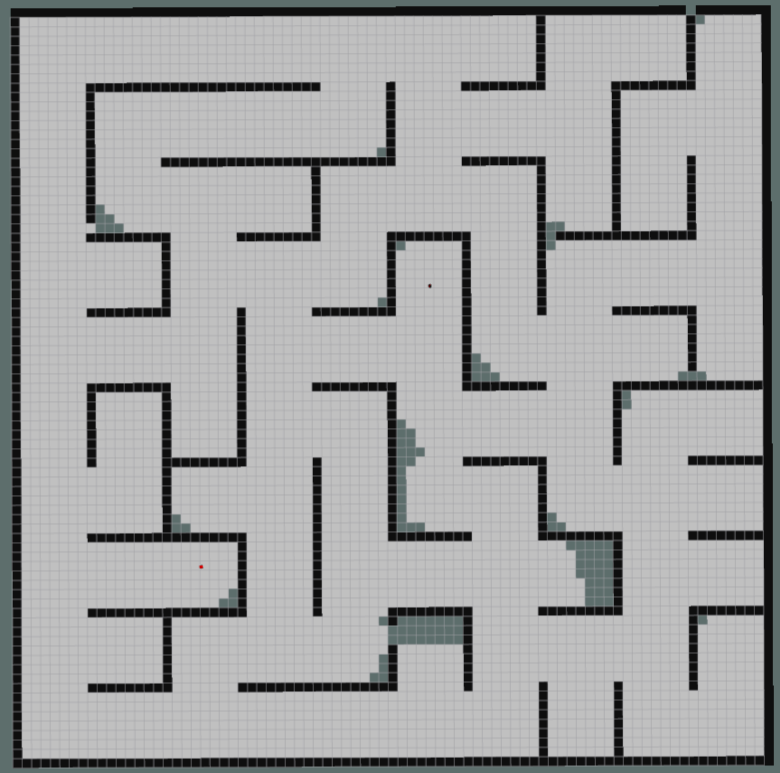
\includegraphics[height=2.5in]{./Imagenes/im.png}
	\caption{Imagen tomada al finalizar un experimento}
	\label{Figura Entornos 7}
\end{figure}

Se realizaron 10 experimentos para cada cantidad de robots, donde cada uno cuenta con una simulación utilizando el estimador de información ganada al momento de calcular la utilidad como se describió en la sección anterior y una simulación utilizando un estimador de costo, donde se tomó por costo la distancia a recorrer. Para poder realizar la simulación con el estimador de costo se modificó la función de utilidad en el código que se había desarrollado para el componente central. Todas las simulaciones se finalizaron al alcanzar el100\% del cubrimiento del mapa y salvo por el estimador utilizado para la distribución de tareas por parte del módulo central, se encuentran en idénticas condiciones.

En dichas simulaciones se registró el cubrimiento acumulado en función del tiempo. En el caso de las simulaciones que se realizaron utilizando el estimador de información ganada, se contabilizo la cantidad de decisiones que el estimador provoco una decisión que hubiera sido distinta si se hubiese tenido en cuneta el estimador de costo. En ambas simulaciones se registró la cantidad de metros recorrida y la eficiencia de la simulación.




\section{First Section}

\subsection{A Subsection Sample}
Please note that the first paragraph of a section or subsection is
not indented. The first paragraph that follows a table, figure,
equation etc. does not need an indent, either.

Subsequent paragraphs, however, are indented.

\subsubsection{Sample Heading (Third Level)} Only two levels of
headings should be numbered. Lower level headings remain unnumbered;
they are formatted as run-in headings.

\paragraph{Sample Heading (Fourth Level)}
The contribution should contain no more than four levels of
headings. Table~\ref{tab1} gives a summary of all heading levels.

\begin{table}
\caption{Table captions should be placed above the
tables.}\label{tab1}
\begin{tabular}{|l|l|l|}
\hline
Heading level &  Example & Font size and style\\
\hline
Title (centered) &  {\Large\bfseries Lecture Notes} & 14 point, bold\\
1st-level heading &  {\large\bfseries 1 Introduction} & 12 point, bold\\
2nd-level heading & {\bfseries 2.1 Printing Area} & 10 point, bold\\
3rd-level heading & {\bfseries Run-in Heading in Bold.} Text follows & 10 point, bold\\
4th-level heading & {\itshape Lowest Level Heading.} Text follows & 10 point, italic\\
\hline
\end{tabular}
\end{table}


\noindent Displayed equations are centered and set on a separate
line.
\begin{equation}
x + y = z
\end{equation}
Please try to avoid rasterized images for line-art diagrams and
schemas. Whenever possible, use vector graphics instead (see
Fig.~\ref{fig1}).

\begin{figure}
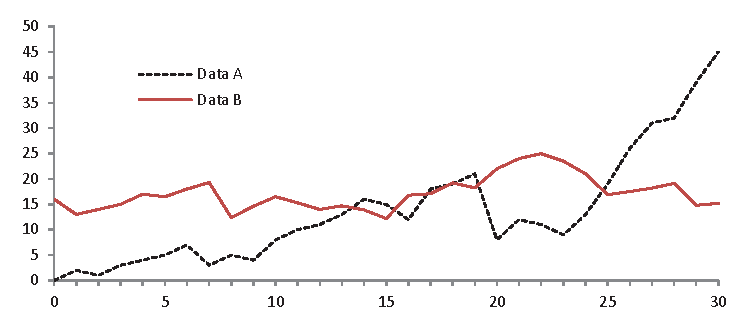
\includegraphics[width=\textwidth]{fig1.eps}
\caption{A figure caption is always placed below the illustration.
Please note that short captions are centered, while long ones are
justified by the macro package automatically.} \label{fig1}
\end{figure}

\begin{theorem}
This is a sample theorem. The run-in heading is set in bold, while
the following text appears in italics. Definitions, lemmas,
propositions, and corollaries are styled the same way.
\end{theorem}
%
% the environments 'definition', 'lemma', 'proposition', 'corollary',
% 'remark', and 'example' are defined in the LLNCS documentclass as well.
%
\begin{proof}
Proofs, examples, and remarks have the initial word in italics,
while the following text appears in normal font.
\end{proof}
For citations of references, we prefer the use of square brackets
and consecutive numbers. Citations using labels or the author/year
convention are also acceptable. The following bibliography provides
a sample reference list with entries for journal
articles~\cite{ref_article1}, an LNCS chapter~\cite{ref_lncs1}, a
book~\cite{ref_book1}, proceedings without editors~\cite{ref_proc1},
and a homepage~\cite{ref_url1}. Multiple citations are grouped
\cite{ref_article1,ref_lncs1,ref_book1},
\cite{ref_article1,ref_book1,ref_proc1,ref_url1}.
%
% ---- Bibliography ----
%
% BibTeX users should specify bibliography style 'splncs04'.
% References will then be sorted and formatted in the correct style.
%
% \bibliographystyle{splncs04}
% \bibliography{mybibliography}
%
\begin{thebibliography}{8}
	
\bibitem{artRef} 
R. Simmons, D. Apfelbaum, W. Burgard, D. Fox, M. Moors, S. Thrun, H. Younes
\textit{Coordination for multi-robot exploration and mapping}. 
AAAI/IAAI, 2000.	
	
\bibitem{onSwitch} 
F.Amigoni, J. Fanfi, A.Longoni
\textit{Online switch of communication modalities for efficient multirobot exploration}. 
European Conference on Mobile Robots (ECMR), 2017.

\bibitem{war} 
S.M. Thayer, M.B. Dias, B. Nabbe, B.L. Digney, M. Hebert, A. Stentz
\textit{Distributed robotic mapping of extreme environments}. 
Mobile Robots XV and Telemanipulator and Telepresence Technologies VII, 2013.

\bibitem{cooperative2017} 
Masehian Ellips, et al.
\textit{Cooperative mapping of unknown environments by multiple heterogeneous mobile robots with limited sensing.}. 
Robotics and Autonomous Systems, Enero 2017
		
\bibitem{Luo} 
Luo R.C., Lai C.C.
\textit{Enriched indoor map construction based on multisensor fusion approach for intelligent service robot}. 
IEEE Trans. Ind. Electron., 2012

\bibitem{lu} 
Lu F., Milios E.
\textit{Robot pose estimation in unknown environments by matching 2d range scans}
J. Intell. Robot. Syst, 1997

\bibitem{fontan} 
M. Fontan and M. Mataric.
\textit{Territorial Multi-Robot Task Division}
IEEE Transactions on Robotics and Automation, 1998.

\bibitem{tool} 
D. Goldberg and M.J. Matarić
\textit{Interference as a Tool for Designing and Evaluating Multi-Robot Controllers}
Proc. AAAI-97, 1997.

\bibitem{metricas} 
Z. Yan , L. Fabresse, J. Laval, N. Bouraqadi.
\textit{Building a ROS-Based Testbed for Realistic Multi-Robot Simulation: Taking the Exploration as an Example}.
2017.

\bibitem{otro} 
K. Singh, K. Fujimura
\textit{Map making by cooperating mobile robots }.
IEEE International Conference on Robotics and Automation, 1993 	

\bibitem{utility}
J.Butzke, M.Likhachev
\textit{Planning for multi-robot exploration with multiple objective utility functions}.
EEE/RSJ International Conference on Intelligent Robots and Systems (IROS), 2011

\bibitem{Visser}
A. Visser and B. Slamet
\textit{Balancing the information gain against the movement cost for multi-robot frontier exploration}.
European Robotics Symposium, 2008

\bibitem{Zlot}
R. Zlot, A. Stentz, M. Dias, and S. Thayer.
\textit{Multi-robot exploration	controlled by a market economy}.
IEEE International Conference on Proceedings, 2002

\bibitem{Gonzalez}
H. H. Gonzalez-Banos and J.-C. Latombe.
\textit{Navigation strategies for exploring indoor environments}.
The International Journal of Robotics Research, 2002

\bibitem{Blach}
T. Balch and R.C. Arkin.
\textit{Communication in Reactive Multiagent Robotic Systems.}.
Autonomous Robots 1, 1994

\bibitem{Yama}
B. Yamauchi.
\textit{A frontier-based approach for autonomous exploration.}.
Computational Intelligence in Robotics and Automation, 1997.

\bibitem{thrun}
S. Thrun.
\textit{Learning Metric-Topological Maps for Indoor	Mobile Robot Navigation.}.
Artificial Intelligence 1, 1998

\bibitem{leo}
J. Leonard, H. Durrant-Whyte and I. Cox. 
\textit{“Dynamic Map Building for an Autonomous Mobile Robot.”}
International Journal of Robotics Research, 1992.

\bibitem{choset}
H. Choset.
\textit{Sensor Based Motion Planning: The Hierarchical Generalized Voronoi Graph}
Ph.D. Thesis, California Institute of Technology, 1996

\bibitem{chino}
Z. Yan, L. Fabresse, J. Laval and N. Bouraqadi
\textit{Team Size Optimization for Multi-robot Exploration}
In Proceedings of the 4th International Conference on Simulation, Modeling, and Programming for Autonomous Robots, 2014
\end{thebibliography}
\end{document}
